% (C) 2020 Diogo Rodrigues
% Licensed under Creative Commons Attribution-NonCommercial-NoDerivatives 4.0 International (CC-BY-NC-ND 4.0)

\documentclass{sope}
\usepackage[english]{babel}
% Metadata
\title{SOPE -- Exam 2015/16}
\author{Diogo Miguel Ferreira Rodrigues \\ \href{mailto:dmfrodrigues2000@gmail.com}{dmfrodrigues2000@gmail.com}}
% Document
\begin{document}

\setcounter{chapter}{15}
\exam{Exam 2015/16}
\question{Question 1}
\questionitem{Item a}
Many mechanisms in modern operatin systems could not be implemented without proper hardware support. Identify the hardware support required to implement the following mechanisms. Explain in one sentence. (\textbf{Note:} if more than one kind of hardware support is needed, identify only one)

\ansseparator

\begin{center}
    \begin{tabular}{p{20mm} | p{131mm}}
        Operating system protection & Kernel/privileged mode and instructions (low-level instructions with unrestricted access to all computer resources) and user mode (has controlled access to computer resources through the OS API)\\ \hline
        CPU scheduling & Dispatcher, which gives a certain process control over the CPU. This involves context commuting, commuting from kernel (mode in which the interrupt was received) to user mode (where the process will run) and setting program counter to correct program address. \\ \hline
        Semaphores & The test\&set instruction, which allows to atomically set and get the previous value of a registry.
    \end{tabular}
\end{center}

\questionitem{Item b}
\textbf{Q1:} User processes can be classified as CPU-bound or I/O-bound. What information can the operating system use to distinguish CUP-bound from I/O-bound processes?\\
\textbf{Q2:} Processor scheduling algorithms generally tend to penalize one of this type of processes. Which one? Why? How can that penalization be enforced?

\ansseparator

\textbf{A1:} CPU-bound processes have a few generally long CPU-bursts, while I/O-bound processes have a lot of short CPU-bursts. This means the operating system can analyse the length and number of CPU-bursts to check if they are CPU-bound or I/O-bound, namely by keeping for example the mean CPU-burst length; if it is short, then the process is I/O-bound, otherwise it is CPU-bound.

The OS can also keep track of the amount of time a process has been blocked waiting for I/O operations, as a I/O-bound process spends most time blocked while waiting for I/O operations to finish.

\textbf{A2:} It depends on the algorithm; FCFS and RR tend to penalize I/O-bound while SJF and SRTF tend to penalize CPU-bound processes. However, assuming all algorithms wish to be as close to the optimal algorithm as possible, they should penalize CPU-bound processes because those consume the most CPU time in general, and the optimal algorithm schedules processes that take less CPU time first so they finish as soon as possible.

Penalties can be implemented using a priority system according to the estimated CPU time required to run the process. In real situations it is hard to estimate this value, so one way is to use a preemptive algorithm that reevaluates the priority of a process every time that process is preempted or blocks (for instance RR, which preempts a process after it consumes a quantum $q$ of time and reevaluates its priority).

\questionitem{Item c}
A car park has a capacity for $N$ cars. Each car takes up an individual spot. Cars wanting to park have to pass a traffic light that is only green when there are free parking spots; in that case cars can enter the park. After entering it, each car must wait for the previous car to choose a free stop to park.

Using semaphores, write the code of process \texttt{car} that simulates this behaviour. Consider the following function operating over semaphores are available: \texttt{init(sem, value)}, \texttt{wait(sem)} and \texttt{signal(sem)}.

\ansseparator

\begin{lstlisting}[language=C]
// In initialization
init(traffic_light, N)  // Capacity of car park
init(choosing_spot, 1)  // Number of cars that can be inside the park
                        // and choosing a free spot
// While running
wait(traffic_light);    // Trying to enter the car park
wait(choosing_spot);    // Waiting for previous car to choose spot
                        // before starting to choose spot
for(int i = 0; i < N; ++i){
    if(is_spot_free(i)){
        take_spot(i);
        break;
    }
}
signal(choosing_spot);  // Done choosing spot, another car can choose
use_spot();
signal(traffic_light);  // Leaving the car park
\end{lstlisting}

\questionitem{Item d}
Consider the following code and the result of an execution.

\begin{center}
    \begin{tabular}{p{91mm} p{0mm} p{56mm}}
        \begin{lstlisting}[language=C,showstringspaces=false]
#include ...
int main(){
  int x;
  if(fork() > 0){
    x = 1;
    printf("&x = %p; x = %d\n", &x, x);
    wait(NULL);
  } else {
    x = 2;
    printf("&x = %p; x = %d\n", &x, x);
  }
  return 0;
}
        \end{lstlisting} & &
        \begin{lstlisting}
&x = 0x7fff62860754; x=1
&x = 0x7fff62860754; x=2
        \end{lstlisting}
    \end{tabular}
\end{center}

\textbf{Q1:} How do you explain that the addresses of variable \texttt{x} are the same in both processes but the values of \texttt{x} are different?

\textbf{Q2:} Is it expectable that results appear always in the same order as in the example above? Justify.

\ansseparator

\textbf{A1:} The presented addresses are virtual addresses, which are references to certain physical memory blocks. Virtual addresses only make sense inside the same process, as different processes have different virtual-physical address translation tables. On forking, the parent's memory is duplicated for the child, so even if the variable has the same virtual address in the parent and child processes, those addresses map to different physical addresses in those processes, meaning that the two processes have two different values for variable \texttt{x}, and they are stored in different virtual addresses.

\textbf{A2:} No, because in this case the order of running processes depends on the state of the CPU and the dispatcher; it may happen that the child is set to execute and the parent continues executing immediately afterwards (and thus will probably write first to stdout), or that the child is initialized and starts running before control is given back to the parent.

\questionitem{Item e}

\textbf{Q1:} Operating systems do not generally care about the existence of deadlocks in user processes. Why? \\
\textbf{Q2:} What is the solution users have to prevent the existence of deadlocks in their processes?

\ansseparator

\textbf{A1:} Because the degree of complexity of evaluating if there is a deadlock in a user process has a very large overhead, it is generally accepted that it is better to let a user process run with the risk of deadlock and assuming a few processes might generate deadlocks once in a while, rather than to check if there can be a deadlock.

\textbf{A2:} The solution is to implement the program so as to make one of the four conditions for deadlocks false (mutual exclusion, hold and wait, non-preemption and circular wait). Generally the easiest option is to prevent circular waits by ordering resources and always request them by that order, meaning that order will be a topological order of the resources/waits graph, and thus it will not have any cycles.

\questionitem{Item f}

\textbf{Q1:} Given the following data, about processes executing in a system, has any of the processes started thrashing? Justify.\\
\textbf{Q2:} Is it advisable to increase the system multiprogramming degree? Justify.

\begin{center}
    \begin{tabular}{c | c | c}
        Process & CPU usage & Pagination disk usage \\ \hline
        P1 & 70\% &  5\% \\
        P2 &  5\% & 85\% \\
        P3 & 10\% &  8\%
    \end{tabular}
\end{center}

\ansseparator

\textbf{A1:} Thrashing happens when a disk uses the pagination disk a lot more often than it uses CPU. This usually means there are a lot of page faults taking place. This is the case for process P2, which is using the pagination disk (85\%) a lot more than the CPU (5\%).

\textbf{A2:} It is not advisable. The multiprogramming degree is the number of programs loaded in principal memory. The fact P2 is thrashing means it already does not have enough frames allocated to it, so the multiprogramming degree is already too high. Further increasing the multiprogramming degree would cause other processes to lose allocated frames, and thus they could also enter thrashing.

\questionitem{Item g}
The execution of command \texttt{ls -laiR} on a certain directory follows. Remember the first column represents the i-node.

\textbf{Q1:} Knowing the directory is \texttt{/home/user1/}, what is the path on which the command was executed?

\textbf{Q2:} Identify the type of entries \texttt{a}, \texttt{b} and \texttt{g} that appear in the listing and point out the access permissions to \texttt{b}.

\textbf{Q3:} Write the shell command that gives execution permission to \texttt{b}, to its owner, keeping the other permissions.

\textbf{Q4:} Say if any of the entries (\texttt{a}...\texttt{g}) has a content which is \underline{certainly} equal. Justify your answer.

\ansseparator

\textbf{A1:} \texttt{/home/user1/SOPE}

\textbf{A2:} \texttt{a} is a directory. \texttt{b} is a regular file. \texttt{g} is a pipe. \texttt{b} has read and write permissions for the owner and group, and read permissions for others.

\textbf{A3:} \texttt{chmod u+x b}

\textbf{A4:} Entries \texttt{c} and \texttt{e} certainly have equal content. This is because \texttt{c} and \texttt{e} are hard links to the same file, which is the file described by i-node 157053.

\question{Question 2}
Consider the following figure that summarizes the arquitecture of a multithreaded, master-slave system, typical of a HTTP server. Requests arrive from the network and are placed in a processing queue. A load balancer reads those requests by order, and assigns them to multiple workers (each worker runs in an independent thread).

\begin{center}
    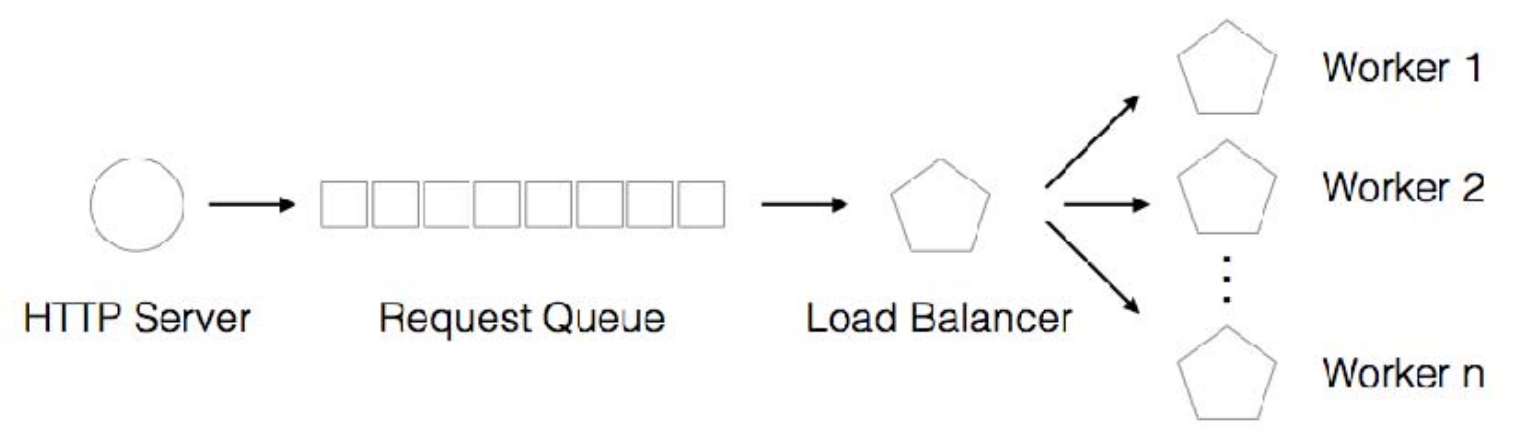
\includegraphics[scale=0.2]{2016N-2}
\end{center}

Also consider the following code skeleton that implements the server (admit needed \texttt{\#include}'s have been made).

\begin{lstlisting}[language=C]
const int NUM_WORKERS = 4;

pthread_t workers[NUM_WORKERS];
pthread_t loadBalancer;

void* dequeueJob();
void* lbEntry(void*p);
void* workerEntry(void*p);
intsetupLB();
intsetupFifos();
intsetupWorkers();
intteardownWorkers();
intteardownLB();
intteardownFifos();
voidlistenHTTPrequests();

int main(int argc, const char * argv[]){
    if(setupFifos()){
        printf("FIFOs setup failed\n");
        return1;
    }
    if(setupWorkers()){
        printf("Worker setup failed\n");
        return 2;
    }
    if(setupLB()){
        printf("LB setup failed\n");
        return 3;
    }
    listenHTTPrequests();
    teardownWorkers();
    teardownLB();
    teardownFifos();
    return 0;
}
\end{lstlisting}

\questionitem{Item a}
Implement function \texttt{setupFifos}, that must create FIFOs with name \texttt{/tmp/myfifoX} where \texttt{X} is an integer identifying the FIFO. Admit there is a FIFO for each worker, and that its identifiers are sequential, starting in 1.

\ansseparator

\begin{lstlisting}[language=C]
int setupFifos(){
    for(int i = 1; i <= NUM_WORKERS; ++i){
        char fifoname[256];
        sprintf(fifoname, "/tmp/myfifo%d", i);
        mkfifo(fifoname, 0777);
    }
    return 0;
}
\end{lstlisting}

\questionitem{Item b}

Implement function \texttt{setupLB} which creates a thread for the load balancer, whose entry function is \texttt{lbEntry}.

\ansseparator

\begin{lstlisting}[language=C]
int setupLB(){
    pthread_create(&loadBalancer, NULL, lbEntry, NULL);
    return 0;
}
\end{lstlisting}

\questionitem{Item c}

Implement function \texttt{setupWorker} that creates a thread for each worker, whose entry funtion is \texttt{workerEntry}. Function \texttt{workerEntry} receives as parameter the identifier of the worker, which is a sequential integer starting in 1.

\ansseparator

\begin{lstlisting}[language=C]
int setupWorkers(){
    for(int i = 0; i < NUM_WORKERS; ++i){
        int *arg = malloc(sizeof(int));
        *arg = i+1;
        pthread_create(&workers[i], NULL, workerEntry, arg);
    }
}
\end{lstlisting}

\questionitem{Item d}
Implement function \texttt{workerEntry}, that should
\begin{enumerate*}[label=(\arabic*)]
    \item open the respective FIFO in read mode,
    \item wait for a message to be sent to it, of type C-string (with null-character), and
    \item write that message to a file with name \texttt{workerX.log}, where \texttt{X} is the worker identifier. For simplicity, consider each worker executes an infinite cycle of message reception
\end{enumerate*}.

\ansseparator

\begin{lstlisting}[language=C]
void* workerEntry(void *p){
    int id = *(int*)p;
    char fifo_name[256];
    sprintf(fifo_name, "/tmp/myfifo%d", id);
    int fifo_fd = open(fifo_name, O_RDONLY);
    char log_name[256];
    sprintf(log_name, "worker%d.log", id);
    int log_fd = open(log_name, O_WRONLY | O_APPEND);
    char message[PIPE_BUF];
    while(1){
        int i = 0;
        while(read(fifo_fd, buf+i, 1) && buf[i] != '\0'){}
        write(log_fd, buf, strlen(buf));
    }
    return NULL;
}
\end{lstlisting}

\questionitem{Item e}
Implement functions \texttt{teardownWorkers} and \texttt{teardownLB} which must assure a good server termination relative to the resources they are associated with.

\ansseparator

\begin{lstlisting}[language=C]
int teardownLB(){
    void *status = NULL;
    if(pthread_join(loadBalancer, &status)) return 1;
    return *(int*)status;
}
int teardownWorkers(){
    void *status = NULL;
    for(int i = 0; i < NUM_WORKERS; ++i){
        if(pthread_join(workers[i], &status)) return 1;
        if(*(int*)status != 0) return 1;
    }
    return 0;
}
\end{lstlisting}

\newpage
\question{Question 3}
Two threads (\texttt{t1} and \texttt{t2}) of the same process need to use the same condition variable. The second thread has a code section that should only execute when a certain condition \texttt{C} is verified (boolean expression). While it is not verified the thread should remain blocked. Elements that can chance the value the expression \texttt{C} evaluates to are modified in the first thread.

\questionitem{Item a}
Knowing thread \texttt{t2} is launched by \texttt{t1}, and that it requires a parameter of type \texttt{info\_t} whose value is generated by calling function \texttt{info\_t get\_info()}, write the lines of code of \texttt{t1} that start executing \texttt{t2}.

\ansseparator

\begin{lstlisting}[language=C]
info_t *info = malloc(sizeof(info_t))
*info = get_info();
pthread_t t2_tid;
pthread_create(&t2_tid, NULL, t2, info);
\end{lstlisting}

\questionitem{Item b}
Write the lines of code that create and initialize the items necessary to use the condition variable.

\ansseparator

\begin{lstlisting}[language=C]
pthread_cond_t  C       = PTHREAD_COND_INITIALIZER ;
pthread_mutex_t C_mutex = PTHREAD_MUTEX_INITIALIZER;
\end{lstlisting}

\questionitem{Item c}
Where in the code should those lines be placed? Justify.

\ansseparator

Those lines should be placed in global scope, before the implementations of \texttt{t1} and \texttt{t2}. That is because declaring variables in global scope is the easiest way of sharing them among threads of the same process.

\questionitem{Item d}
The internal scheme of the two threads is the one that follows.

\begin{center}
    \begin{tabular}{l | l}
        \texttt{t1} & \texttt{t2} \\ \hline
        \texttt{initializations\_1;} & \texttt{initializations\_2;} \\
        \texttt{...} & \texttt{...} \\
        \texttt{A;} & \texttt{B;} \\
        \texttt{...} & \texttt{...} \\
        \texttt{finalizing\_1;} & \texttt{finalizing\_2;}
    \end{tabular}
\end{center}

In block \texttt{A} the condition \texttt{C} can be changed. Block \texttt{B} can only be executed if \texttt{C} is verified. While it is not verified, \texttt{t2} must remain blocked.

Write for both threads the code that uses the condition variable, mentioning where you would place it in the scheme, so as to obtain the mentioned functionality.

\ansseparator

\begin{center}
    \lstset{
        numbers=none,
        showlines=true
    }
    \begin{tabular}{l | l}
        \texttt{t1} & \texttt{t2} \\ \hline \\
        \begin{minipage}{75mm}\begin{lstlisting}[language=C]
// Placed instead of A in t1
while(1){
  pthread_mutex_lock(&C_mutex);
  A;
  if(condition())
    pthread_cond_signal(&C);
  pthread_mutex_unlock(&C_mutex);
}
        \end{lstlisting}\end{minipage} &
        \begin{minipage}{75mm}\begin{lstlisting}[language=C]
// Placed instead of B in t2
pthread_mutex_lock(&C_mutex);
while(!condition())
  pthread_cond_wait(&C,&C_mutex);
B;
pthread_mutex_unlock(&C_mutex);


        \end{lstlisting}\end{minipage}
    \end{tabular}
\end{center}

\questionitem{Item e}
Admit now that there are several instances of \texttt{t2} waiting for condition \texttt{C} and it is intended that all of them execute \texttt{B} when condition \texttt{C} is verified. Rewrite the code of \texttt{t1} so as to allow that behaviour.

\ansseparator

\begin{lstlisting}[language=C]
// initializations_1
pthread_t t2_tids[NTHREADS];
for(int i = 0; i < NTHREADS; ++i){
    info_t *info = malloc(sizeof(info_t))
    *info = get_info();
    pthread_create(&t2_tids[i], NULL, t2, info);
}
// Placed instead of A in t1
while(1){
    pthread_mutex_lock(&C_mutex);
    A;
    if(condition())
        pthread_cond_broadcast(&C);
    pthread_mutex_unlock(&C_mutex);
}
\end{lstlisting}

\questionitem{Item f}
If instead of two threads there were two processes using the same condition variable, say if it would be necessary or not to create other items and modify their initialization. Justify.

\ansseparator

It would be necessary to create shared memory to store all synchronization mechanisms. The easiest way would be to create a structure containing \texttt{C} and \texttt{C\_mutex}, allocate shared memory with the size of that structure and then open it in both processes. Then it would be used as usual, except uses of \texttt{C} would be replaced by \texttt{data->C} and \texttt{C\_mutex} by \texttt{data->C\_mutex}.

\begin{lstlisting}[language=C]
// global, in t1 and t2
#define SHM_NAME "/tmp/shm"
typedef struct {
    pthread_cond_t C;
    pthread_mutex_t C_mutex;
} shared_data;
shared_data *data = NULL;
\end{lstlisting}
\begin{center}
    \begin{tabular}{c c c}
        \begin{minipage}{73mm}\begin{lstlisting}[language=C]
// t1
// main, beginning
int shm_fd = shm_open(
    SHM_NAME,
    O_CREAT | O_RDWR,
    0777
);
ftruncate(
    shm_fd,
    sizeof(shared_data)
);
data = (shared_data*)mmap(
    NULL,
    sizeof(shared_data),
    PROT_READ|PROT_WRITE,
    MAP_SHARED,
    shm_fd,
    0
);
// ...
        \end{lstlisting}\end{minipage} & &
        \begin{minipage}{73mm}\begin{lstlisting}[language=C]
// t2
// main, beginning
int shm_fd = shm_open(
    SHM_NAME,
    O_RDWR,
    0777
);




data = (shared_data*)mmap(
    NULL,
    sizeof(shared_data),
    PROT_READ|PROT_WRITE,
    MAP_SHARED,
    shm_fd,
    0
);
// ...
        \end{lstlisting}\end{minipage}
    \end{tabular}
\end{center}
\begin{lstlisting}[language=C]
// main end, in t1 and t2
munmap(data, sizeof(shared_data));
shm_unlink(SHM_NAME);
\end{lstlisting}

\end{document}